\chapter{Methodology: Development Journey}\label{ch:methodology}

This chapter narrates the complete development journey of our system---from initial technology evaluation through four iterations of the ZK circuit, three generations of contract architecture, custom blockchain development, and mobile app challenges. Unlike a sanitized methodology section, we present the \textit{actual} path: what we tried, what failed, why it failed, and how each failure informed the next iteration.

\section{Technology Selection Process}

\subsection{ZK Circuit Language: Circom to Noir}

\subsubsection{Initial Attempt: Circom}

Our first implementation attempt used Circom~\cite{belles2022circom}, the most established ZK circuit DSL. We implemented a basic Merkle membership proof in Circom with the following structure:

\begin{lstlisting}[language=Java, caption={Initial Circom circuit attempt (abandoned).}]
template VoteMembership(depth) {
    signal input nullifier;
    signal input secret;
    signal input siblings[depth];
    signal input pathIndices[depth];
    signal output nullifierHash;
    signal output root;
    
    component hasher = Poseidon(2);
    hasher.inputs[0] <== nullifier;
    hasher.inputs[1] <== secret;
    // ... Merkle path verification
}
\end{lstlisting}

\textbf{Problems encountered with Circom}:
\begin{enumerate}
    \item \textbf{R1CS constraint model}: Circom compiles to Rank-1 Constraint Systems, which are less expressive than Plonkish arithmetization. Custom gates (needed for efficient Poseidon) require awkward workarounds.
    \item \textbf{Trusted setup requirement}: Circom targets Groth16, requiring a per-circuit trusted setup ceremony via \texttt{snarkjs powers of tau}. For a university project, coordinating a multi-party ceremony was impractical.
    \item \textbf{JavaScript-centric toolchain}: The \texttt{snarkjs} library generates proofs in Node.js. On React Native's Hermes engine, BigInt operations were unsupported, requiring polyfills that increased proof time from 15s to 90s.
    \item \textbf{Template verbosity}: Circom requires explicit signal wiring for every operation, making the circuit logic spread across 200+ lines for our relatively simple proof.
\end{enumerate}

\subsubsection{Migration to Noir}

Noir~\cite{aztec2024noir}, developed by Aztec Labs, offered a compelling alternative:
\begin{itemize}
    \item \textbf{Rust-like syntax}: High-level, readable code that compiles to ACIR (Abstract Circuit Intermediate Representation)
    \item \textbf{UltraHonk backend}: No trusted setup; the keccak transcript eliminates ceremony coordination
    \item \textbf{Barretenberg (bb.js)}: WASM-ready prover that runs in WebView contexts
    \item \textbf{Built-in Poseidon}: Native stdlib support for Poseidon over BN254
    \item \textbf{Concise expression}: Our entire circuit fits in $\sim$30 lines of Noir
\end{itemize}

The migration from Circom to Noir reduced our circuit from 210 lines to 28 lines while simultaneously eliminating the trusted setup requirement. This was the first major architectural decision that shaped the entire system.

\begin{figure}[H]
\centering
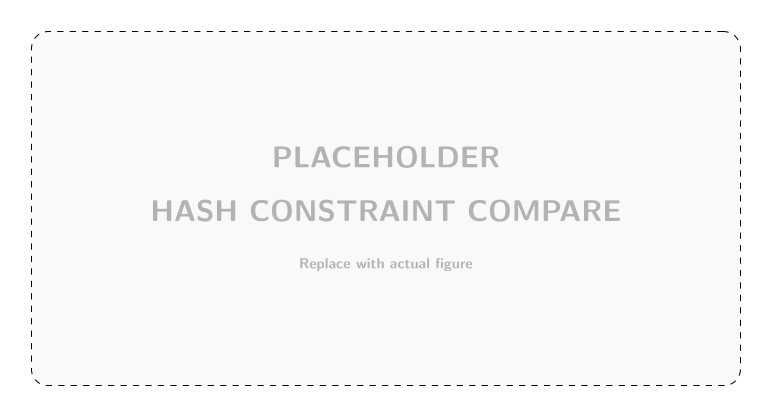
\includegraphics[width=0.85\textwidth]{Images/fig_hash_constraint_compare.png}
\caption{Constraint count comparison between Circom+Groth16 and Noir+UltraHonk for equivalent circuit logic.}
\label{fig:hash-constraint}
\end{figure}

\subsection{Hash Function: SHA-256 to Poseidon}

\subsubsection{SHA-256 Attempt}

Our earliest prototype used SHA-256 for all hashing (commitments, Merkle nodes, nullifiers). This choice seemed natural---SHA-256 is the most widely deployed hash function and has extensive security analysis.

\textbf{What we observed}: The Circom SHA-256 circuit required approximately 25,000 constraints per hash invocation. With a depth-16 Merkle tree requiring 17 hash computations (1 commitment + 16 path nodes), the total circuit size exceeded 425,000 constraints. Proof generation on a mobile device was estimated at 3--5 minutes---completely unacceptable for user experience.

\subsubsection{Why SHA-256 Fails in Arithmetic Circuits}

SHA-256 operates on 32-bit words with bitwise operations (XOR, AND, rotation). In an arithmetic circuit over $\mathbb{F}_p$, each bit operation requires:
\begin{itemize}
    \item Range checks to ensure values are boolean
    \item Decomposition/recomposition between field elements and bit arrays
    \item Simulated bitwise operations using arithmetic ($a \oplus b = a + b - 2ab$ in $\mathbb{F}_p$)
\end{itemize}

\subsubsection{Poseidon Solution}

Poseidon's algebraic design uses only field multiplications and additions---operations that are \textit{native} to the arithmetic circuit. The S-box $x \mapsto x^5$ is a single multiplication gate in UltraHonk.

\textbf{Result}: Circuit size dropped from 425,000 to approximately 5,100 constraints. Proof generation time decreased from minutes to 15--30 seconds in WebView WASM.

\subsection{Blockchain Platform: Ethereum to L2 to Custom}

\begin{figure}[H]
\centering
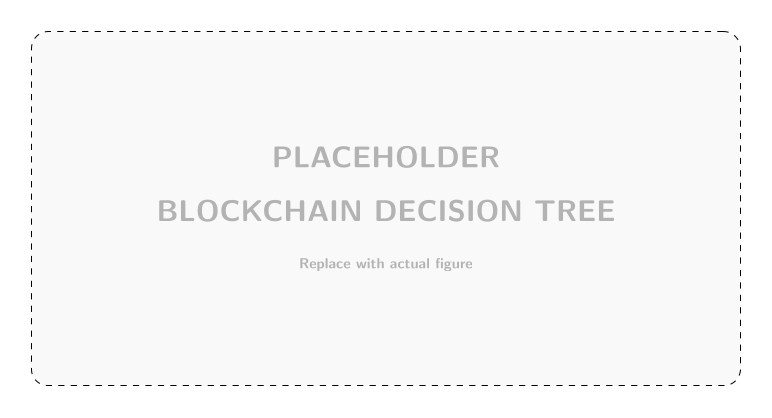
\includegraphics[width=0.85\textwidth]{Images/fig_blockchain_decision_tree.png}
\caption{Decision tree showing our evaluation of blockchain platforms and why we built a custom chain.}
\label{fig:blockchain-decision}
\end{figure}

\subsubsection{Phase 1: Ethereum Mainnet}

Initial development targeted Ethereum mainnet using Hardhat for local testing. We successfully deployed and tested all contracts on the Hardhat local node.

\textbf{Blocking issue}: Gas costs. A single \texttt{vote()} transaction costs approximately 350,000 gas ($\sim$\$15 at 30 gwei). For 16 million voters, this represents an impossible economic barrier. Even with gas sponsorship, the total cost would exceed \$240 million.

\subsubsection{Phase 2: Layer 2 Evaluation}

We evaluated several L2 solutions:

\begin{table}[H]
\centering
\caption{L2 platform evaluation for voting workload.}
\label{tab:l2-eval}
\begin{tabular}{|l|l|l|l|}
\hline
\textbf{Platform} & \textbf{Vote Cost} & \textbf{Finality} & \textbf{Blocking Issue} \\
\hline
Arbitrum & \$0.05--0.20 & 7 days (L1) & Still costs money \\
\hline
Optimism & \$0.05--0.15 & 7 days (L1) & Still costs money \\
\hline
Base & \$0.01--0.05 & 7 days (L1) & Still costs money \\
\hline
Polygon PoS & \$0.001 & 2 hours & Reorg risk \\
\hline
\end{tabular}
\end{table}

\textbf{Fundamental insight}: Any public chain---L1 or L2---charges fees. Even \$0.001 per vote $\times$ 16M voters = \$16,000. More critically, it creates a dependency on cryptocurrency markets and wallet funding that is inappropriate for a national election.

\subsubsection{Phase 3: Custom Go Blockchain}

The decision to build a custom blockchain was driven by three non-negotiable requirements:
\begin{enumerate}
    \item \textbf{Zero cost}: Voting must be economically free
    \item \textbf{Deterministic finality}: No reorgs or probabilistic confirmation
    \item \textbf{Sovereignty}: No dependency on external networks or token economics
\end{enumerate}

The custom blockchain embeds go-ethereum's EVM package, executing the \textit{same compiled Solidity bytecode} as our Hardhat tests. This architectural choice means our 54 unit tests validate the exact code running in production.

\subsection{Mobile Framework: Flutter to React Native}

\begin{figure}[H]
\centering
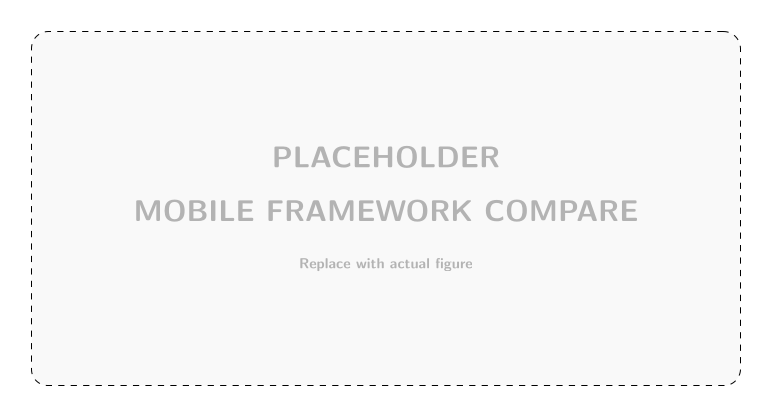
\includegraphics[width=0.85\textwidth]{Images/fig_mobile_framework_compare.png}
\caption{Mobile framework evaluation against our ZK voting requirements.}
\label{fig:mobile-framework}
\end{figure}

\subsubsection{Flutter Evaluation}

Flutter (Dart) was initially considered for its cross-platform capabilities and native performance. However:
\begin{itemize}
    \item No mature EVM library for Dart (web3dart is unmaintained)
    \item No equivalent of \texttt{expo-secure-store} with biometric gating
    \item WebView integration is less mature (no \texttt{react-native-webview} equivalent for WASM proving)
    \item Smaller ecosystem for blockchain-related packages
\end{itemize}

\subsubsection{React Native (Expo) Selection}

React Native with Expo SDK 54 was selected for:
\begin{itemize}
    \item \textbf{viem}: Production-grade EVM interaction library with TypeScript types
    \item \textbf{expo-secure-store}: Hardware-backed keychain with biometric authentication
    \item \textbf{expo-local-authentication}: Unified biometric API (fingerprint + face)
    \item \textbf{WebView}: Mature react-native-webview for hosting WASM bb.js prover
    \item \textbf{poseidon-lite}: JavaScript Poseidon implementation for commitment generation
\end{itemize}

\section{ZK Circuit Evolution}

Our circuit went through four major iterations, each addressing failures discovered in the previous version.

\subsection{Iteration 1: Basic Membership (Failed)}

\begin{figure}[H]
\centering
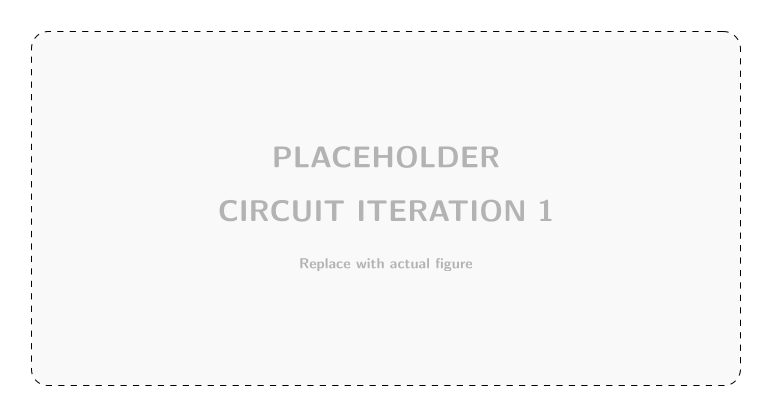
\includegraphics[width=0.85\textwidth]{Images/fig_circuit_iteration_1.png}
\caption{Circuit iteration 1: basic Merkle membership without vote binding or nullifier constraints.}
\label{fig:circuit-v1}
\end{figure}

The first iteration proved only Merkle membership:
\begin{lstlisting}[language=Java, caption={Circuit v1: basic membership (incomplete).}]
fn main(
    root: pub Field,
    nullifier: Field, secret: Field,
    index: Field, siblings: [Field; 16],
) {
    let commitment = poseidon2([nullifier, secret]);
    let computed_root = merkle_root(commitment, siblings, index);
    assert(computed_root == root);
}
\end{lstlisting}

\textbf{Failure}: The vote was not part of the proof. An attacker observing the mempool could extract the valid proof and submit it with a different vote value. The vote was passed as a separate contract parameter with no cryptographic binding.

\subsection{Iteration 2: Vote Binding Added (Partially Failed)}

We added the vote as a public input, binding it into the proof:
\begin{lstlisting}[language=Java, caption={Circuit v2: added vote binding.}]
fn main(
    nullifier_hash: pub Field,
    root: pub Field,
    vote: pub Field,  // NEW: bound into proof
    // ... same private inputs
)
\end{lstlisting}

\textbf{Partial failure}: The nullifier hash was computed \textit{off-chain} and passed as public input without being constrained to match the private nullifier. A malicious voter could submit someone else's nullifier hash while proving with their own secrets---the circuit would not catch the mismatch.

\subsection{Iteration 3: Nullifier Constraint (Subtle Bug)}

We added the nullifier hash verification:
\begin{lstlisting}[language=Java, caption={Circuit v3: nullifier constraint added.}]
assert(poseidon1([nullifier]) == nullifier_hash);
\end{lstlisting}

\textbf{Subtle bug}: The Merkle path used big-endian bit decomposition for the index, but the on-chain LeanIMT tree used little-endian ordering. Proofs verified locally but failed on-chain because the computed root differed when traversing left/right children in reversed order.

\textbf{Diagnosis}: This took 3 days to identify. We generated proofs that passed the Noir prover but failed HonkVerifier on-chain. The error was ``InvalidRoot''---the proof was technically valid, but proved membership in a differently-ordered tree.

\subsection{Iteration 4: Final Correct Circuit}

\begin{figure}[H]
\centering
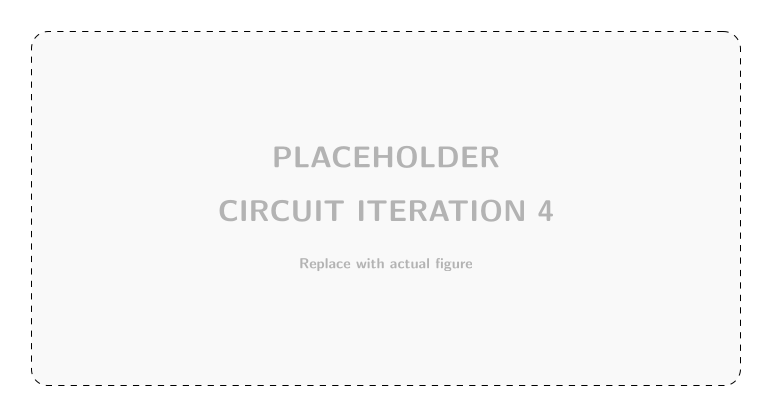
\includegraphics[width=0.85\textwidth]{Images/fig_circuit_iteration_4.png}
\caption{Circuit iteration 4 (final): all constraints correct, matching on-chain tree ordering.}
\label{fig:circuit-v4}
\end{figure}

The final circuit uses \texttt{index.to\_le\_bits()} (little-endian), matching the LeanIMT on-chain implementation:

\begin{lstlisting}[language=Java, caption={Final Noir circuit (v4) with all constraints.}]
fn main(
    nullifier_hash: pub Field,
    root: pub Field,
    vote: pub Field,
    depth: pub u32,
    nullifier: Field,
    secret: Field,
    index: Field,
    siblings: [Field; 16],
) {
    // 1. Nullifier binding
    assert(poseidon1([nullifier]) == nullifier_hash);
    
    // 2. Commitment derivation
    let commitment = poseidon2([nullifier, secret]);
    
    // 3. Merkle membership (little-endian index bits)
    let index_bits = index.to_le_bits();
    let computed = binary_merkle_root(
        hash_2, commitment, depth, index_bits, siblings
    );
    assert(computed == root);
    
    // 4. Vote range check (8-bit)
    let _vote_bits: [u1; 8] = vote.to_le_bits();
}
\end{lstlisting}

\section{Smart Contract Architecture Evolution}

\subsection{Version 1: Monolithic Contract}

\begin{figure}[H]
\centering
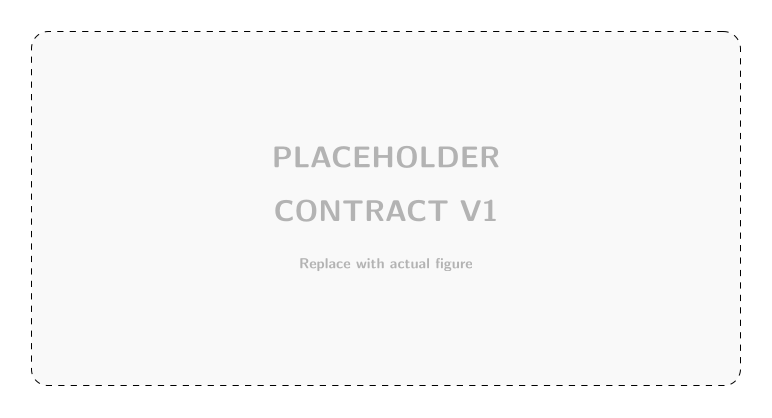
\includegraphics[width=0.85\textwidth]{Images/fig_contract_v1.png}
\caption{Contract v1: single monolithic contract handling all divisions and all logic.}
\label{fig:contract-v1}
\end{figure}

The first contract version was a single \texttt{Voting.sol} that managed all 160 divisions internally:
\begin{lstlisting}[language=Java, caption={Contract v1: monolithic (abandoned).}]
mapping(uint256 divisionId => MerkleTree) trees;
mapping(uint256 divisionId => Phase) phases;
mapping(uint256 divisionId => mapping(uint256 => uint256)) voteCounts;
\end{lstlisting}

\textbf{Problems}:
\begin{itemize}
    \item Gas cost scaled with division count for any lookup
    \item Single point of failure: a bug in one division's logic affected all
    \item Access control complexity: every function needed a divisionId parameter
    \item Deployment bytecode exceeded Ethereum's 24KB contract size limit
\end{itemize}

\subsection{Version 2: Manual Multi-Contract}

We manually deployed separate Voting contracts and tracked them off-chain. This worked but required:
\begin{itemize}
    \item Manual coordination of 160 deployments
    \item Off-chain registry of contract addresses
    \item No on-chain national aggregation
    \item Manual GN officer assignment (error-prone)
\end{itemize}

\subsection{Version 3: Factory Pattern (Final)}

\begin{figure}[H]
\centering
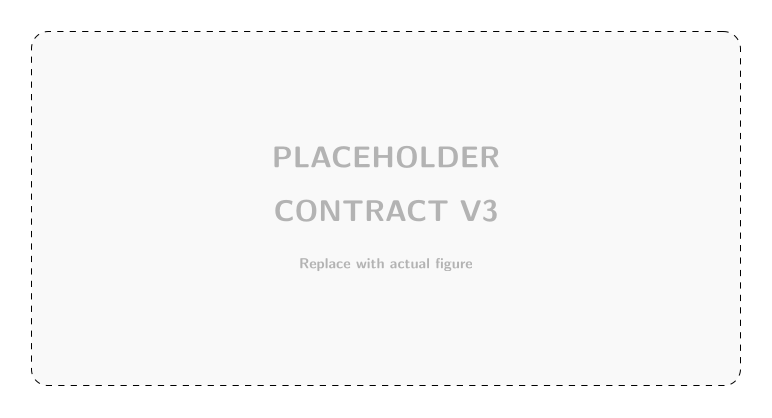
\includegraphics[width=0.85\textwidth]{Images/fig_contract_v3.png}
\caption{Contract v3 (final): ElectionRegistry factory pattern with per-division Voting instances.}
\label{fig:contract-v3}
\end{figure}

The final architecture uses the factory pattern with three key contracts:
\begin{enumerate}
    \item \texttt{ElectionRegistry}: Factory that deploys and manages Voting instances
    \item \texttt{Voting}: Per-division election state machine (isolated)
    \item \texttt{NicRegistry}: Global NIC de-duplication across all divisions
\end{enumerate}

This provides isolation (a bug in one division cannot affect others), on-chain aggregation (national results computed by summing across divisions), and administrative delegation (GN officers per division).

\section{Custom Blockchain Development Challenges}

\subsection{EVM Embedding}

\textbf{Challenge}: Running Solidity contracts inside a custom blockchain required embedding the go-ethereum EVM. This is not a documented use case---go-ethereum is designed as a standalone node, not an embeddable library.

\textbf{What we tried}: Initially, we attempted to use go-ethereum's \texttt{ethclient} package to connect to an external node. This worked but defeated the purpose of a sovereign chain.

\textbf{Final approach}: We imported go-ethereum's \texttt{core/vm} package directly, creating a custom \texttt{StateDB} implementation backed by BoltDB:

\begin{lstlisting}[language=Java, caption={EVM embedding in Go (simplified).}]
// Create EVM context
blockCtx := vm.BlockContext{
    BlockNumber: new(big.Int).SetUint64(blockNum),
    Time:        uint64(time.Now().Unix()),
    GasLimit:    16_000_000,
}

// Execute contract call
evm := vm.NewEVM(blockCtx, txCtx, stateDB, chainConfig, vmConfig)
ret, _, err := evm.Call(caller, contractAddr, calldata, gasLimit, value)
\end{lstlisting}

\textbf{Key insight}: The EVM itself is stateless---it reads/writes through the StateDB interface. By implementing this interface ourselves, we could use any backing store (BoltDB in our case) while executing the exact same bytecode as Ethereum mainnet.

\subsection{Gasless Execution Model}

\textbf{Challenge}: Standard EVM execution charges gas, deducting from the sender's balance. In our gasless model, voters have zero balance.

\textbf{Solution}: We set the gas limit to 16M for all transactions and never deduct gas costs. The EVM still \textit{meters} gas (for DoS protection and infinite loop prevention) but we do not subtract from any account balance. The authority (election commission) implicitly sponsors all execution.

\subsection{StateDB Implementation}

The most complex challenge was implementing go-ethereum's \texttt{StateDB} interface, which includes:
\begin{itemize}
    \item Account balance/nonce management
    \item Contract code storage/retrieval
    \item Storage slot read/write (per-contract key-value store)
    \item Log (event) emission
    \item Snapshot/revert for atomic transactions
    \item Suicide (selfdestruct) handling
\end{itemize}

Our implementation uses BoltDB buckets for persistence, with an in-memory dirty cache for pending state changes that are flushed on block commit.

\subsection{BN254 Precompile for Proof Verification}

\textbf{Challenge}: The HonkVerifier contract calls the BN254 pairing precompile at address \texttt{0x08}. Go-ethereum includes these precompiles, but they must be explicitly registered in the chain configuration.

\textbf{What failed initially}: We used a minimal chain config without precompile registration. HonkVerifier calls succeeded in Hardhat (which registers all precompiles by default) but reverted with ``execution reverted'' on our custom chain.

\textbf{Fix}: Register all Istanbul-era precompiles in our custom EVM configuration, including ecRecover (0x01), SHA-256 (0x02), RIPEMD-160 (0x03), identity (0x04), modexp (0x05), ecAdd (0x06), ecMul (0x07), and ecPairing (0x08).

\section{Mobile Development Challenges}

\subsection{Hermes Engine BigInt Crisis}

\begin{figure}[H]
\centering
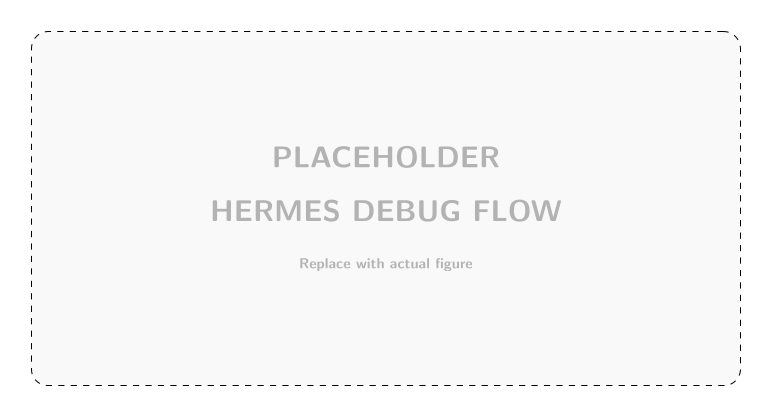
\includegraphics[width=0.85\textwidth]{Images/fig_hermes_debug_flow.png}
\caption{Debugging flow for the Hermes BigInt incompatibility: from cryptic error to WebView solution.}
\label{fig:hermes-debug}
\end{figure}

\textbf{The problem}: React Native uses the Hermes JavaScript engine (not V8). Hermes does not support native BigInt. Our entire cryptographic pipeline (Poseidon, field arithmetic, proof generation) relies on BigInt for 254-bit field element arithmetic.

\textbf{What we observed}: Importing \texttt{poseidon-lite} crashed immediately with ``BigInt is not defined''. The \texttt{viem} library (which uses BigInt for transaction encoding) also failed.

\textbf{Attempted solutions}:
\begin{enumerate}
    \item \textbf{BigInt polyfill (JSBI)}: Added JSBI polyfill, but poseidon-lite uses BigInt literals (\texttt{21888...n}) which cannot be polyfilled at the syntax level.
    \item \textbf{babel-plugin-transform-bigint}: Transforms BigInt syntax to JSBI calls. Partially worked for our code but broke library internals that used \texttt{BigInt()} constructor.
    \item \textbf{ethers.js v5}: Used its bundled BigNumber polyfill. Worked for basic operations but could not be used with poseidon-lite.
\end{enumerate}

\textbf{Final solution}: A hybrid architecture:
\begin{itemize}
    \item \textbf{poseidon-lite}: Used in a React Native WebView (which runs V8/JavaScriptCore with native BigInt support)
    \item \textbf{viem}: Used with legacy transaction signing (manually constructing RLP-encoded transactions without BigInt-dependent auto-estimation)
    \item \textbf{ZK proof generation}: Entirely in WebView via bb.js WASM
\end{itemize}

\subsection{WebView ZK Proving Architecture}

\begin{figure}[H]
\centering

\includegraphics[width=0.85\textwidth]{Images/fig_webview_proof_arch.png}
\caption{WebView-based proof generation architecture: React Native passes witness data to an embedded WebView running bb.js WASM.}
\label{fig:webview-arch}
\end{figure}

The WebView proving pipeline works as follows:
\begin{enumerate}
    \item React Native constructs the circuit witness (using field arithmetic in WebView)
    \item Witness is serialized and passed to the proving WebView via \texttt{postMessage}
    \item WebView loads bb.js WASM module and compiled ACIR circuit
    \item bb.js generates the UltraHonk proof (15--30 seconds)
    \item Proof bytes are returned to React Native via \texttt{onMessage} callback
    \item React Native constructs the transaction calldata from proof bytes
\end{enumerate}

\subsection{Biometric Authentication Integration}

\textbf{Challenge}: \texttt{expo-local-authentication} provides biometric prompts, but \texttt{expo-secure-store} has its own authentication gate. Coordinating these two systems to provide a seamless single-prompt experience required careful state management.

\textbf{Key decision}: We set \texttt{requireAuthentication: true} on sensitive keystore items (private key, nullifier, secret) but \texttt{false} on non-sensitive items (address, division selection, voted flags). This means accessing secrets triggers a single OS-level biometric prompt, while reading public state does not interrupt the user.

\subsection{Legacy Transaction Signing}

\textbf{Challenge}: viem's \texttt{sendTransaction} uses EIP-1559 gas estimation internally, which calls BigInt operations. On Hermes, this crashes.

\textbf{Solution}: We manually construct legacy (pre-EIP-1559) transactions:
\begin{lstlisting}[language=Java, caption={Manual legacy transaction construction for Hermes compatibility.}]
// Build raw transaction manually (no BigInt auto-estimation)
const tx = {
  to: contractAddress,
  data: encodeFunctionData(...),
  gasLimit: "0x" + (500000).toString(16),
  gasPrice: "0x0",  // gasless chain
  nonce: "0x" + nonce.toString(16),
  chainId: 31337,
};
const signed = await signTransaction(privateKey, tx);
const hash = await sendRawTransaction(signed);
\end{lstlisting}

\section{Integration Challenges}

\subsection{Poseidon Field Mismatch}

\textbf{The bug}: When testing end-to-end (mobile $\to$ blockchain $\to$ on-chain verification), proofs generated on mobile were rejected on-chain with ``InvalidProof''.

\textbf{Root cause}: The \texttt{poseidon-lite} npm package uses a slightly different round constant derivation than the Noir stdlib's Poseidon. Both are ``Poseidon over BN254'' but produce different outputs for the same input due to different MDS matrices.

\textbf{Detection}: We generated test vectors---hashing the same value in both environments and comparing outputs. The mismatch was immediately visible.

\textbf{Fix}: We ensured both the mobile app and the Noir circuit use the exact same Poseidon parameterization (the one from circomlibjs/poseidon-lite). The Noir stdlib's \texttt{std::hash::poseidon} matched this parameterization, but we needed to verify by generating matching test vectors.

\subsection{Bit Ordering: The Three-Day Bug}

\textbf{Symptom}: Proofs for tree index 0 and 1 verified correctly, but index 2 and above failed on-chain.

\textbf{Investigation}: For index 0 (binary: 000...0) and index 1 (binary: 000...1), the bit ordering (big-endian vs. little-endian) produces the same path traversal. Starting at index 2 (binary: 10 LE vs. 01 BE), the difference manifests.

\textbf{Resolution}: Changed circuit to use \texttt{to\_le\_bits()} matching the LeanIMT library's convention of treating the least-significant bit as the first tree level.

\subsection{Public Input Ordering}

\textbf{The problem}: The HonkVerifier expects public inputs in a specific order: \texttt{[nullifier\_hash, root, vote, depth]}. The order is determined by the Noir compiler's output, which follows the declaration order in the circuit function signature.

\textbf{What happened}: We initially passed inputs as \texttt{[root, nullifier\_hash, vote, depth]} (alphabetical order in our contract code). The verifier silently verified against wrong values and returned false.

\textbf{Lesson}: Public input ordering must exactly match the circuit's function signature parameter order. We added a comment in the contract code documenting this requirement.

\section{Development Methodology}

\subsection{Iterative Bottom-Up Approach}

We followed an iterative bottom-up methodology rather than a waterfall approach:

\begin{enumerate}
    \item \textbf{Cryptographic Core First}: ZK circuit correctness is the foundation. We invested 6 weeks perfecting the circuit before writing any application code.
    \item \textbf{Contract Testing}: 54 unit tests validate all contract behavior before integration. Tests are run after every change.
    \item \textbf{Vertical Slices}: Each feature was implemented as a complete vertical slice (mobile $\to$ API $\to$ contract $\to$ verification) before moving to the next.
    \item \textbf{Continuous Integration Testing}: End-to-end proof generation and verification tested after each circuit or contract change.
\end{enumerate}

\subsection{Tools and Environment}

\begin{table}[H]
\centering
\caption{Development tools and their roles in our workflow.}
\label{tab:dev-tools}
\begin{tabular}{|l|l|l|}
\hline
\textbf{Tool} & \textbf{Version} & \textbf{Purpose} \\
\hline
Nargo & 1.0.0-beta.3 & Noir circuit compilation and testing \\
\hline
Hardhat & 2.22 & Solidity compilation, testing, deployment \\
\hline
Go & 1.21 & Custom blockchain implementation \\
\hline
Expo & SDK 54 & React Native mobile app development \\
\hline
Next.js & 14.x & Web application framework \\
\hline
Barretenberg (bb) & 0.82.x & Proof generation and verification \\
\hline
Yarn & 4.13.0 & Monorepo package management \\
\hline
\end{tabular}
\end{table}

\section{Summary of Key Decisions}

\begin{table}[H]
\centering
\caption{Summary of technology decisions with rationale.}
\label{tab:decisions-summary}
\resizebox{\textwidth}{!}{%
\begin{tabular}{|l|l|l|p{5cm}|}
\hline
\textbf{Decision} & \textbf{Rejected} & \textbf{Selected} & \textbf{Key Rationale} \\
\hline
Circuit DSL & Circom & Noir & No trusted setup, readable syntax, WASM prover \\
\hline
Hash function & SHA-256 & Poseidon & 83$\times$ fewer constraints in circuit \\
\hline
Proof system & Groth16 & UltraHonk & No ceremony, faster mobile proving \\
\hline
Blockchain & Ethereum/L2 & Custom Go & Zero gas fees, sovereignty, PBFT finality \\
\hline
Mobile & Flutter & React Native & viem, expo-secure-store, WebView WASM \\
\hline
Contracts & Monolithic & Factory & Isolation, scalability, delegation \\
\hline
Key storage & AsyncStorage & expo-secure-store & Hardware TEE, biometric gate \\
\hline
Signing & EIP-1559 & Legacy tx & Hermes BigInt incompatibility workaround \\
\hline
\end{tabular}%
}
\end{table}

Each decision was arrived at through practical experience with the rejected alternative---not theoretical analysis alone. This empirical approach ensured that our final architecture addresses real, observed problems rather than hypothetical concerns. Chapter~\ref{ch:circuit} details the final ZK circuit implementation that emerged from these four iterations.
